\documentclass[a4paper]{scrartcl}

\usepackage{float}
\usepackage{tikz}
\usetikzlibrary{arrows,automata}
\usepackage{pgf}
\usepackage[utf8]{inputenc} % this is needed for umlauts
\usepackage[ngerman]{babel} % this is needed for umlauts
\usepackage[T1]{fontenc}    % this is needed for correct output of umlauts in pd
\usepackage{amssymb}
\usepackage{amsmath}
\usepackage{mathrsfs}
\usepackage{dsfont}
\usepackage{graphicx}
\usepackage{fancyhdr}
\usepackage{lastpage}
\usepackage{imakeidx}
\setlength{\parskip}{\medskipamount}
\setlength{\parindent}{0pt}
\usepackage{enumitem}
\usepackage{hyperref}

%%%%%%%%%%%%%%%%%%%%%%%%
% Kopf- und Fusszeilen %
%%%%%%%%%%%%%%%%%%%%%%%%
\pagestyle{fancy}
\lhead{
        Maximilian Roth
}
\chead{Logik-Tutorat Lösungen Blatt 3\\}
\rhead{
        \today{} \\
        Seite \thepage{} von \pageref{LastPage}\\
        
}
\lfoot{}
\cfoot{}
\rfoot{} 

%%%%%%%%%%%%%%%%%%%%%%%%
% Anfang des Dokuments %
%%%%%%%%%%%%%%%%%%%%%%%%

\begin{document}
\section*{Disclaimer}%
\label{sec:disclaimer}
Auch in diesem Dokument können sich Fehler befinden!\\
Sie sind nicht die Musterlösung der Aufgaben, sondern selbst erstellte Lösungen.\\

Als generelle Lektüre kann ich nur das Skript von Markus Junker aus dem WS 17/18 empfehlen:\\
\url{http://home.mathematik.uni-freiburg.de/junker/skripte/InfoLogik.pdf}\\
Hier ist vieles sehr genau und verständlich erklärt.

\section*{}%
\label{sec:aufgabe_1}

    Siehe auch 

    \begin{figure}[H]
        \centering
        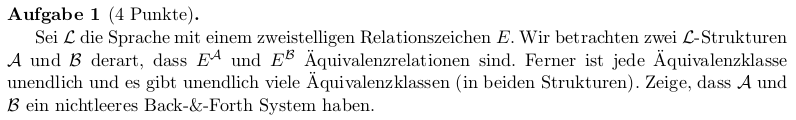
\includegraphics[scale=0.6]{./A-1.png}
        \label{fig:}
    \end{figure} 

    \underline{Beweis:}\\
    Wir sollen zeigen, dass es ein nicht leeres Back and Forth System gibt, also müssen wir uns zuerst eines aussuchen.\\
    \\Hierfür empfiehlt es sich zuerst mit folgendem S anzufangen:\\
    $S = \{F: \mathfrak{C} \rightarrow \mathfrak{D} \mathscr{L}-Isomorphismus| \mathfrak{C} \subset \mathfrak{A}, \mathfrak{D} \subset \mathfrak{B},
    \text{ wobei  }\mathfrak{C}, \mathfrak{D} \text{ endlich erzeugt}\}$ ist.\\
    Mit $\mathfrak{C} \subset \mathfrak{A}$ ist gemeint, dass $\mathfrak{C}$ Unterstruktur von $\mathfrak{A}$ ist.\\

    \\Zeigen wir also nun, dass S ein nichtleeres Back and Forth System ist. 

    \begin{itemize}
        \item S ist nichtleer\\
            Sei gegeben: $\mathfrak{C} = (\{c\}, \{E^\mathfrak{C}\}), \mathfrak{D} = (\{d\}, \{E^\mathfrak{D}\})$\\
            \\Dann gilt, dass $F: \{c\} \rightarrow \{d\}, c \mapsto d$ Isomorphismus ist
            \\(Die von \{c\} und \{d\} erzeugten Mengen sind wieder \{c\} bzw. \{d\} und offensichtlich endlich erzeugt),\\
            da F klar bijektiv und E in beiden Strukturen Äquivalenzerelartion ist, womit F auch starker $\mathscr{L}$-Hom. ist.\\

        \item S ist Back & Forth System\\
            \begin{itemize}
                \item Back:\\
                    

            \end{itemize}
    \end{itemize}
    



\section*{}%
\label{sec:aufgabe_2}

    \begin{figure}[H]
        \centering
        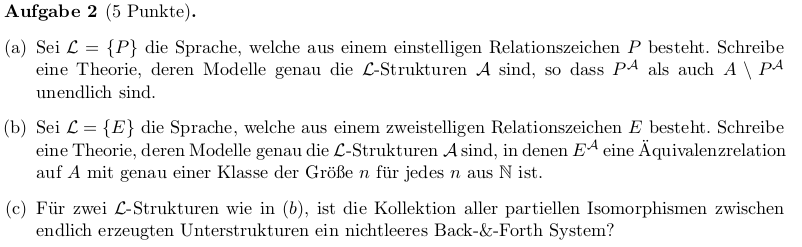
\includegraphics[scale=0.6]{./A-2.png}
        \label{fig:}
    \end{figure}

    Eine Theorie ist eine Menge T von $\mathscr{L}$-Aussagen.

    \begin{itemize}
        \item a)\\
            $T = A_1 \cup A_2$\\
            $A_1 = \{\exists x_1 \dots \exists x_n (\bigwedge_{i \neq j}(\neg x_i \doteq x_j \land P(x_i,x_j))) | n \in \mathds{N}\}$\\
            Also keine zwei Variablen sind gleich und alle n sind in Relation\\
            $\Rightarrow$ Es gibt min n Elemente in P $\forall n \in \mathds{N}$\\
            $\Rightarrow$ Es gibt unendlich viele Elemente in P\\
            \\$A_2 = \{\exists x_1 \dots \exists x_n (\bigwedge_{i \neq j}(\neg x_i \doteq x_j \land \neg P(x_i,x_j))) | n \in \mathds{N}\}$\\
            Es sind also mindestens n Elemente nicht in P $\forall n \in \mathds{N}$\\
            $\Rightarrow$ Es gibt unendlich viele Elemente, die nicht in P liegen.\\
            \\Aus $T = A_1 \cup A_2$ folgt, dass unendlich viele Elemente in P sind und unendlich viele es nicht sind.\\

        \item b)\\

    \end{itemize}


\section*{}%
\label{sec:aufgabe_3}

    \begin{figure}[H]
        \centering
        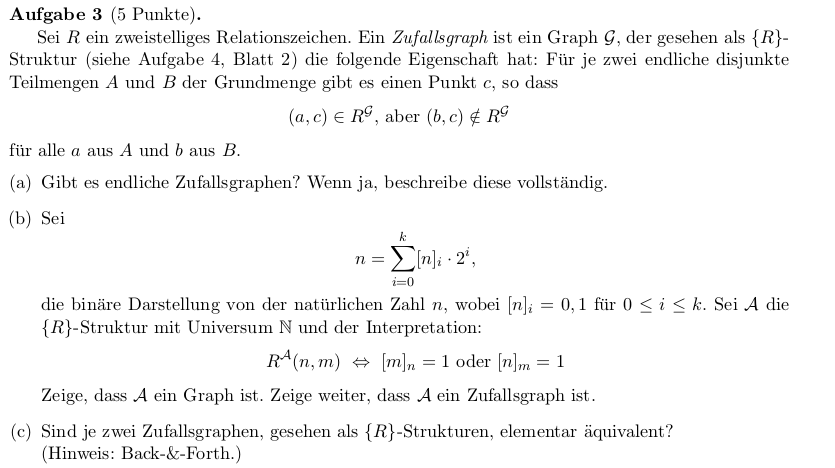
\includegraphics[scale=0.6]{./A-3.png}
        \label{fig:}
    \end{figure}

\section*{}%
\label{sec:aufgabe_4}

    \begin{figure}[H]
        \centering
        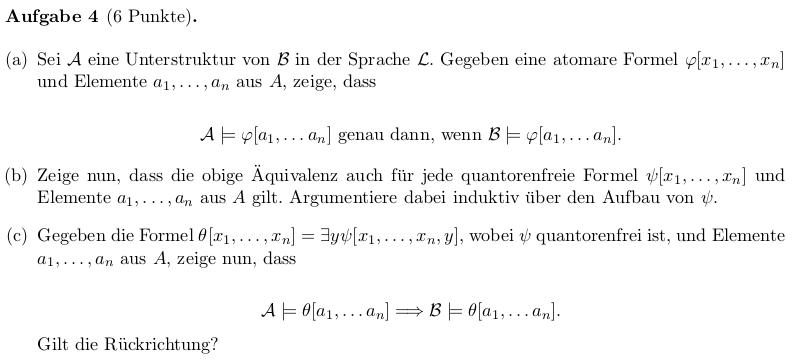
\includegraphics[scale=0.6]{./A-4.png}
        \label{fig:}
    \end{figure}


\section*{Aufbau Back \& Forth}%
\label{sec:aufbau_back_forth}
    Das finden eines nichtleeren Back \& Forth Systems S wird dazu genutzt, um zu zeigen, dass zwei Strukturen elementar äquivalent sind.
    \begin{figure}[H]
        \centering
        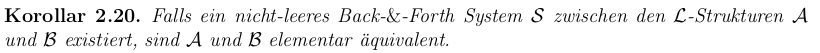
\includegraphics[scale=0.6]{./B&F-EA.png}
        \label{fig:}
    \end{figure}

    Das heißt, wenn eine eine partielle elementare Abbildung von der einen in die andere Struktur existiert:
    
    \begin{figure}[H]
        \centering
        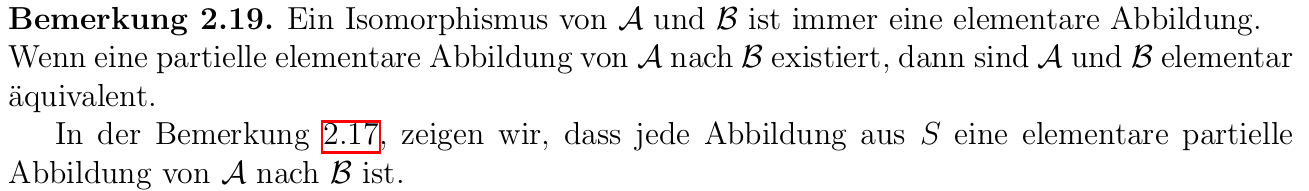
\includegraphics[scale=0.3]{./B&F-PEA.png}
        \label{fig:}
    \end{figure}

    Was wiederum der fall ist, wenn folgendes gilt:

    \begin{figure}[H]
        \centering
        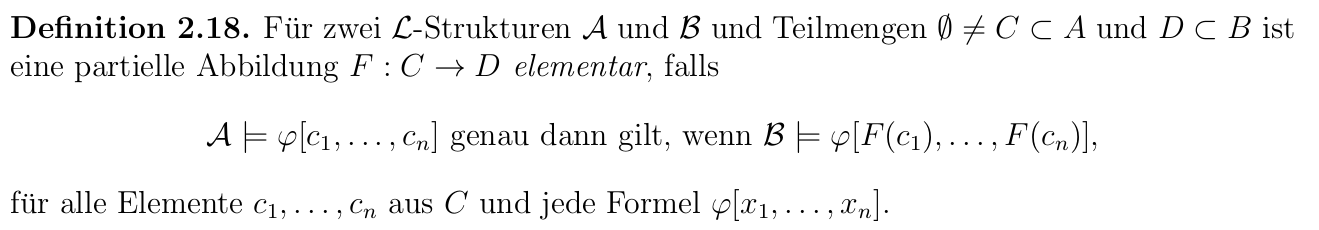
\includegraphics[scale=0.3]{./B&F-E.png}
        \label{fig:}
    \end{figure}

    Also suchen wir stets (falls nicht gegeben) eine Kollektion S mit den Eigenschaften:\\

    $S = \{F: \mathfrak{C} \rightarrow \mathfrak{D} \mathscr{L}-Isomorphismus| \mathfrak{C} \subset \mathfrak{A}, \mathfrak{D} \subset \mathfrak{B},
    \text{ wobei  }\mathfrak{C}, \mathfrak{D} \text{ endlich erzeugt}\}$ ist.\\
    Mit $\mathfrak{C} \subset \mathfrak{A}$ ist gemeint, dass $\mathfrak{C}$ Unterstruktur von $\mathfrak{A}$ ist.\\

    Falls dieses S kein nichtleers Back \& Forth System ist, können wir ein weiter eingeschränktes S suchen.\\
    Hier hängt die Einschränkung vom konkreten Fall ab, schaut einfach, wo das Problem für euer erstes S lag.\\
    Es kann natürlich aus sein, dass keins existiert, wenn dies der Fall ist seht ihr das aber in der Regel schnell.\\

    Habt ihr ein S, dann zeigt die nötigen Eigenschaften:\\
    \begin{itemize}
        \item S ist nichtleer\\
        \item S ist Back \& Forth System\\
            \framebox{Back:}\\
                Sei $F \in S$, also F bildet von C nach D isomorph ab und gelte $d \in D\backslash Im(F)$.\\
                Dann muss für dieses beliebige c gelten, dass ein F' existiert mit:\\
                \\$F': C\cup \{c\} \rightarrow D \cup \{d\} $
    \end{itemize}



\end{document}

